\begin{figure}[htb]
	\centering
	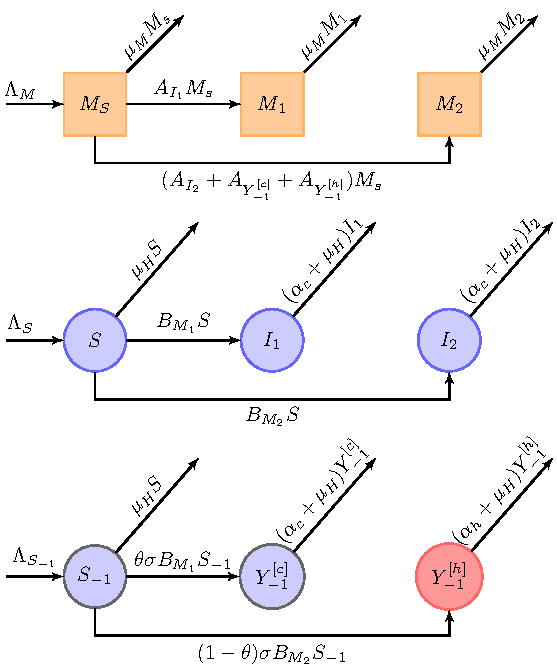
\includegraphics[width=\linewidth]{disiase_flow.pdf}
	\caption{Flow diagram of model \eqref{eqn:model_two_strains}}.
	\label{fig:disiaseflow}
\end{figure}
%
\begin{table}[h!]
	\begin{center}
		\begin{tabular}{rl}
			\toprule
			Symbol		&	\multicolumn{1}{c}{Meaning}
			\\
			\midrule
			$M_S$
				& Number of susceptible mosquitoes.
			\\
			$M_1$, $M_2$
				&
				 Number of infected mosquitoes with virus
				\\
				& 
				serotype \ac{DENV-1} or \ac{DENV-2}.
			\\
			$S$
				&
				Susceptible host population which, 
				\\
				& never has acquired dengue.
			\\
			$S_{-1}$
			&
				Susceptible host population 
				which is immune to
			\\
			&
				serotype $1$.
			\\
			$I_1$, $I_2$
			&
				First time infected host population by 
			\\
				& serotype $1$ and $2$, respectively.
			\\
				$Y_{-1}^{[h]}$,
				$Y_{-1}^{[c]}$
				&
				Second time infected host population with 
				\\
				&
				serotype 2, with \ac{DHF} and \ac{DCF}, 
                \\
                &
                respectively.
			\\
		\bottomrule
		\end{tabular}
	\end{center}
	\caption{
		Meaning of variables. 
		Here we omit the explicit dependence of
		time.
	}\label{tbl:variable_description}
\end{table}
